\newpage

\chapter{Мотивация и постановка задачи}
\label{ch:chapter_1}

\section{Диаграммы связей}
\label{sec:mindmaps}
Диаграмма связей представляет собой древовидную структуру, пример на
рис.~\ref{pic:mindmap}.

\begin{figure}[h!]
  \centering
  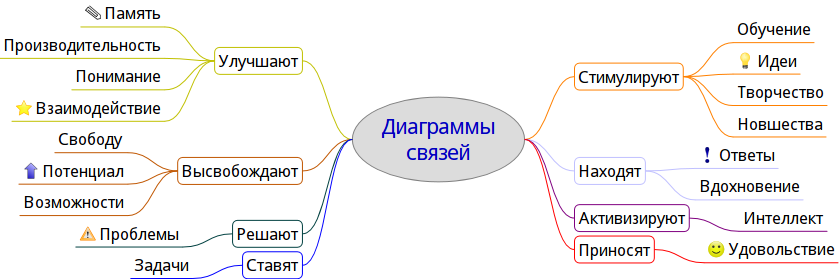
\includegraphics[width=1\linewidth]{mindmap}
  \caption{Пример диаграммы связей}
  \label{pic:mindmap}
\end{figure}

Диаграмма связи состоит из узлов и соединительных линий между ними. Зачастую,
подобная информация лучше воспринимается чем обычный текст. Оформление диаграммы
связей играет большую роль в её восприятии и осознании. Множество ключевых идей
может быть выделено среди всех остальных, используя атрибуты узла или дуг, к
примеру, выделить схожие идеи одинаковым цветом или поставить иконку напротив
некоторых из них. Также существует возможность скрыть некоторые узлы, дабы
сконцентрироваться на требуемой части диаграммы. Чем больше доступных
способов оформления, тем более точно могут быть выражены ассоциативные связи
между узлами, что способствует процессу ассоциативного мышления.


\section{Описание проекта HiveMind}
\label{sec:project_summary}
Мобильные устройства получили большое распространение в современном мире.
Зачастую, приложением, предназначенным для использования на персональном
компьютере, почти невозможно пользоваться на мобильных устройствах. Специфика
мобильных устройств, по сравнению с персональным компьютерами, заключается в
малом разрешении экрана и наличии альтернативных средств ввода. Данные различия
требуют абсолютно иного подхода к построению пользовательских интерфейсов на
мобильных устройствах. Множество людей пользуются мобильными устройствами вне
дома и персональными компьютерами у себя дома. Пользователь использует множество
операционных систем: Windows, Linux, MacOS на настольных компьютерах и Maemo,
Android, MeeGo на мобильных устройствах. Пользователь нуждается в том, чтобы
необходимое ему приложение было доступно под все виды используемых им платформ.
Данный факт ставит перед разработчиками приложений абсолютно новую задачу  ''---
разработка кроссплатформенных приложений с интерфейсом оптимизированным под
настольные и мобильные платформы \cite{hivemind-8th-fruct}.

Существует множество приложений для редактирования диаграмм связи (FreeMind,
Xmind, Vym, iMindMap и т.д.) и веб сервисов в сети интернет (MindMeister,
Mind42, Mindomo и т.д.). К сожалению многие из них платные, другие же,
бесплатные, имеют малую функциональность и лишь немногие имеют поддержку
совместного редактирования диаграмм связи.

Главной целью проекта HiveMind является разработка редактора удовлетворяющего
вышенаписанным требованиям: кроссплатформенность, богатая функциональность,
поддержка функций совместного редактирования.

Основные возможности приложения HiveMind:
\begin{itemize}
\item Чтение и запись файлов в формате FreeMind.
\item Отображение диаграмм связей и навигация по ним.
\item Интерфейс, оптимизированный для настольных и мобильных устройств.
\item Интернационализация.
\item Кроссплатформенность (Поддержка Windows, Linux, Maemo, MeeGo).
\item Использование клавиатуры и сенсорного дисплея.
\end{itemize}


\section{Используемый инструментарий}
\label{sec:toolkit}
Приложение HiveMind написано на языке программирования Python с использованием
библиотеки Qt.

Qt "--- Кросс-платформенный фрэймворк используемый для разработки ПО
~\cite{qt4}. Широко используется для построения приложений с графическим
интерфейсом, так и с интерфейсом командной оболчочки. Изначально, библиотека Qt,
написана на C++, но может быть использована на других язык программирования
используя соотвествующие <<привязки>>. Данная библиотека обладает широкой
функциональностью и имеет множество модулей, обеспечивающий работу с 3D
графикой, веб и мультимедиа контентом, базами данных, сетью и т.д.

Python "--- Интерпретируемый, высокоуровневый язык программирования общего
назначения ~\cite{python}. Он нацелен на быстроту написания и легкую читаемость
кода, обладает понятным и минималистичным синтаксисом. Python имеет поддержку
следующих парадигм программирования: объектно-ориентированное, функциональное,
процедурное, аспектно-ориентированное, императивное. Из особенностей языка
следует отметить дианмическую типизацию, автоматическим управлением памятью,
полную поддержку метапрограммирования и механизм обработки исключений. С данным
языком поставляется большая и многофункциональная библиотека, являющаяся одной
из сильных сторон языка. Помимо всего прочего язык поддерживает написание
внешних модулей на языках C и C++. Интерпретаторы языка Python доступны под
множеством операционных систем.

PyQt "--- набор <<привязок>> фреймворка Qt для языка программирования Python.
PyQt реализует более чем 440 классов и 6000 методов библиотеки Qt, включающих в
себя классы для построения графического интерфейса пользователя, работы с БД,
сетью, XML, SVG и т.д. PyQt лицензирован под двумя лицензиями: GPL и
коммерческой, что позволяет бесплатно использовать его в проектах с открытым
исходным кодом.

Приложение HiveMind является кроссплатформенным и работает под следующими
операционными системами: Windows, Linux, Meego, Maemo. ОС MeeGo ориентирована на
устройства на базе нетбуков, планшетов и ноутбуков, ОС Maemo на мобильные
устройства, в то время как Linux и Windows на настольные компьютеры и ноутбуки.
Каждые из целевых платформ имеют разные форм-факторы, устройства ввода и
соединение с сетью.


\section{Концепция совместного редактирования диаграмм связи}
\label{sec:collaborative_mindmapping}
В общем виде, процесс совместного редактирования диаграмм должен выглядеть
следующим образом. Один пользователь с установленным приложением HiveMind в
любой момент может открыть доступ к своей диаграмме связи. Другой пользователь
подключается к диаграмме связи данного человека и автоматически получает её
актуальную копию, после чего оба пользователя начинают совместное
редактирование. Для того чтобы предоставить различные сценарии
совместного взаимодействие, на сервере должна быть возможность изменять права
участников и режимы доступа карте. Далее будут перечислены возможные сценарии
совместного взаимодействия.

Пользователь создаёт диаграмму связи и начинает её редактирование, используя
мобильное устройство, ноутбук или персональный компьютер. В процессе
редактирования пользователь решает показать свою работу другу (к примеру, для
получения помощи). Для того чтобы сделать данное действие возможным, он
открывает доступ к своей диаграмме. В данном случае ноутбук или мобильное
устройство пользователя работает как сервис, доступный из локальной сети или
интернет. Другой пользователь подключается к диаграмме связи и автоматически
получает актуальную версию диаграммы. Далее оба пользователя начинают совместное
редактирование диаграммы. Количество взаимодействующих участников неограниченно,
поэтому другие пользователи также могут участвовать в совместной работе.
Изменения, совершаемые каждым из участников, незамедлительно посылаются
остальным участникам.

Следующий сценарий использования совместного редактирования диаграмм связи может
быть полезен при представлении докладов. К примеру, докладчик имеет
дополнительные материалы, такие как: план презентации, краткий обзор речи
выстпуление или ссылки на дополнительные ресурсы. Докладчик оформляет данные
материалы в виде диаграммы связи и открывает к ней доступ. Используя HiveMind
cлушатели подключаются к диаграмме связи, выложенной докладчиком, используя свои
мобильные устройства или нетбуки. Таким образом слушатели получают материалы
подготовленные докладчиком, а также все изменения, сделанные докладчиком в
процессе выстпуления и позволяющие более ясно предоставить материал доклада.

Диаграмма связи также может содержать материалы для дискуссии в реальном
времени. В данном случае она может быть использована как лекционная доска с
иерархической структурой, на которую каждый участник может заносить свои идеи,
комментарии или мнения. Главное преимущество такого рода обсуждений с
исполльзованием HiveMind то, что все данные имеют иерархическую структуру и
доставляются всем участникам почти мгновенно.

Пользователь может хранит на диаграмме связи свою личную информацию, поэтому,
открывая доступ к диаграмме связи, он должен иметь возможность ограничить
возможность присоединения к диаграмме только избранному кругу лиц. Также он
должен иметь возможность контролировать права доступа участников на
редактирование. К примеру, при выступлении двух докладчиков перед аудиторией,
необходимо разрешить редактирование диаграммы только выстпуающим и
запретить всем остальным.


\section{Постановка задачи}
\label{sec:problem_statement}
Задача заключается в том, чтобы добавить в проект HiveMind возможность
совместного редактирования диаграмм. Существует множество способов организовать
сетевое взаимодействие. Но в данном случае накладывается ряд ограничений:

\begin{itemize}
\item Сетевая архитектура должна быть построена поверх уже существующего
приложения.
\item Ограничения платформ на которых выполняется приложение.
\item Архитектура должна полностью удовлетворять концепции совместного
редактирования.
\end{itemize}

Необходимо выбрать соответствующие технологии и инструментарий для построения
сетевой архитектуры приложения с учетом вышеназванных ограничений. Данная
архитектура должна быть разработана с оглядкой на уже имеющуюся структуру и
особенности приложения.
